\documentclass[pdflatex,11pt]{aghdpl}

\usepackage[polish]{babel}
\usepackage[utf8]{inputenc}
\usepackage[T1]{fontenc}

% dodatkowe pakiety
\usepackage{enumerate}
\usepackage{pdfpages}
\usepackage{afterpage}
\usepackage{pdflscape}
%\usepackage{rotating}

\graphicspath{{./img/}}
%\usepackage{subfigure} %kilka obrazkow w ramach jednego figure

%------------------------- STRONA TYTUŁOWA -------------------------

\author{Marta~Drabarczyk, Krzysztof~Kutt, Michał~Nowak}
\titlePL{Księgarnia internetowa \textbf{WhaToRead}}
\thesistypePL{Wzorce Projektowe}
\date{2012}
\departmentPL{Katedra Automatyki}
\facultyPL{Wydział Elektrotechniki, Automatyki, Informatyki i Elektroniki}
\setlength{\cftsecnumwidth}{10mm}

%------------------------- DOKUMENT START -------------------------

\begin{document}

\titlepages

\tableofcontents
\clearpage

%------------------------- OGÓLNY OPIS SYSTEMU -------------------------

\chapter{Ogólny opis systemu}

\section{Cel systemu}

Celem projektu było stworzenie prostego systemu informatycznego obsługującego księgarnię internetową z możliwościami zarządzania książkami i kategoriami oraz składania zamówień. W projekcie wykorzystano wzorce projektowe opisane w dalszej części dokumentacji.

%-------------------------

\section{Udziałowcy}

Właścicielami systemu będą firmy prowadzące księgarnie internetowe, zarówno mniejsze jak i większe, gdyż nasz system łatwo skaluje się do dowolnej ilości użytkowników i książek.

Grupę użytkowników wewnętrznych stanowią pracownicy prowadzący bieżącą działalność księgarni: zarządzają aktualną listą książek i kategorii oraz realizują zamówienie składane przez użytkowników.

Użytkownikami zewnętrznymi systemu są klienci księgarni internetowej.

%-------------------------

\section{Granice systemu}

Jedyną granicę systemu stanowi strona internetowa, zapewniająca dostęp do wszystkich funkcjonalności systemu.

%-------------------------

\section{Lista możliwości}

Dla wszystkich:
\begin{enumerate}
\item Rejestracja
\item Logowanie
\item Przeglądanie książek
\item Wyszukiwanie książek
\item Ocenianie książek
\end{enumerate}

Dla klientów:
\begin{enumerate}
\item Przeglądanie i zmiana danych
\item Składanie zamówień
\end{enumerate}

Dla pracowników:
\begin{enumerate}
\item Dodanie/modyfikacja/usunięcie kategorii
\item Dodanie/modyfikacja/usunięcie książki
\item Przeglądanie i zmiana statusów zamówień złożonych przez użytkowników
\end{enumerate}


%------------------------- ANALIZA DZIEDZINY -------------------------

\chapter{Analiza dziedziny}

\section{Produkty}
\begin{itemize}
\item ID produktu
\item Nazwa
\item Opis
\item Cena
\item ID Kategorii
\item Zdjęcie
\item Ilość ocen
\item Suma ocen
\item ilość produktów (na stanie)
\end{itemize}

\section{Kategorie produktów}
\begin{itemize}
\item ID
\item Nazwa
\item Opis
\end{itemize}

\section{Komentarze}
\begin{itemize}
\item ID produktu
\item ID użytkownika
\item Komentarz
\end{itemize}

\section{Zamówienia}
\begin{itemize}
\item ID zamówienia
\item ID klienta
\item dane klienta
\item lista ID produktów
\item Forma dostawy
\item Forma płatności
\item Stan zamówienia
\end{itemize}

\section{Użytkownicy}
\begin{itemize}
\item ID użytkownika
\item Imię
\item Nazwisko
\item Adres
\item Telefon
\item Mail
\end{itemize}


%------------------------- SPECYFIKACJA WYMAGAŃ -------------------------

\chapter{Specyfikacja wymagań}

\section{Przypadki użycia}

\begin{figure}[hbt]
\centering
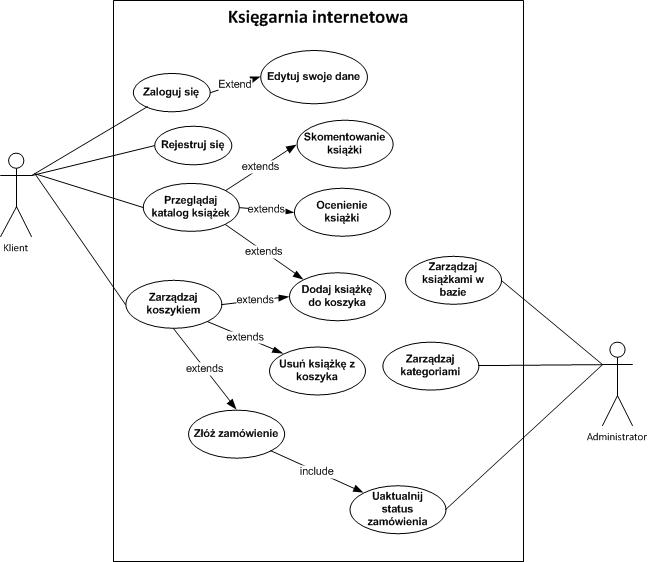
\includegraphics[width=\textwidth]{useCase}
\caption{Diagram przypadków użycia}
\label{fig:useCase}
\end{figure}

\clearpage

%-------------------------

\section{Wybrane funkcjonalności}

\begin{enumerate}
\item Każdy produkt reprezentowany w systemie posiada swoją nazwę, opis, zdjęcie i cenę. Jest dostępna również możliwość oceny danego produktu przez klientów zarówno poprzez skalę punktową, jak i wpisanie komentarza.
\item Podział produktów na kategorie (np. Książki dla dzieci / Książki dla dorosłych / Podręczniki / Czasopisma), które można dowolnie usuwać, bądź dodawać w zależności od aktualnych potrzeb.
\item System posiada funkcjonalność koszyka, do którego klienci mogą dodawać wybrane produkty, celem późniejszego złożenia zamówienia. Koszyk jest przechowywany w ramach aktualnej sesji.
\item Możliwość zakładania kont w serwisie. Dzięki temu klient ma dostęp do historii swoich zamówień i nie musia wpisywać swoich danych przy każdym zamówieniu, gdyż są one pobierane z jego konta.
\item Po poprawnym złożeniu zamówienia, klient otrzymuje mail z informacjami o tym zamówieniu (m.in. numer identyfikacyjny), zaś samo zamówienie pojawia się na liście aktywnych zamówień, dostępnej dla pracowników księgarni.
\item Obsługiwane przez system możliwości płatności to: gotówka przy odbiorze, przelew tradycyjny i karta kredytowa.
\end{enumerate}


%------------------------- WZORCE PROJEKTOWE -------------------------

\chapter{Wzorce projektowe}

\section{Model dziedziny [1.1.2]}

Jeden obiekt odpowiada jednemu wierszowi w tabeli.

\textbf{Wykorzystanie:} Moduł ,,użytkownik'' odpowiada jednemu wierszowi w tabeli ,,użytkownicy''.

%-------------------------

\section{Active record [1.2.3]}

Obiekty, które poza danymi zawierają również metody do obsługi tych danych.

\textbf{Wykorzystanie:} Obiekt użytkownik, poza informacjami takimi jak id, imię, nazwisko itd, posiada kilka wbudowanych metod(index, new ,create, show, edit, update, destroy - dostępne we wszystkich metodach Ruby on Rails)

%-------------------------

\section{Data mapper [1.2.4]}

Oddziela bazę danych od obiektów aplikacji, jego zadaniem jest wymiana informacji pomiędzy nimi.

%\textbf{Wykorzystanie:} X

%-------------------------

\section{Klucz główny [1.1.1]}

Pole pozwalające jednoznacznie zidentyfikować obiekt. Przechowywanie identyfikatora pobranego z bazy w obiekcie, co usprawni operacje wyszukiwania i zapisu. Wybór tego wzorca wiąże się z decyzją projektową o typie klucza i jego powtarzalności w obrębie bazy danych.

\textbf{Wykorzystanie:} Pola ,,id'' w każdej tabeli

%-------------------------

\section{Mapowanie klucza obcego [1.1.2]}

Odwzorowuje relacje pomiędzy obiektami. W ruby wykonywane poprzez użycie: has\_one, belongs\_to itd.

\textbf{Wykorzystanie:} Wiersz w tabeli produkty posiada pole ,,kategoria'' odwołujące się do pola ,,id'' w tabeli kategorie produktów.

%-------------------------

\section{Tabela asocjacji [1.1.3]}

Dodatkowa tabela pomagająca odwzorować relację wiele do wielu

\textbf{Wykorzystanie:} Jedna książka może znajdować się w wielu zamówieniach, podobnie jak jedno zamówienie może zawierać wiele książek. Konieczne jest stworzenie pomocniczej tabeli zawierającej tylko informację o id\_zamowienia i id\_ksiazki.

%-------------------------

\section{obiekt zapytania [1.2.2]}

Obiekt odpowiedzialny za generowanie zapytań do bazy SQL w zależności od klasy obiektu oraz jego pól

\textbf{Wykorzystanie:} Polecenie order.find(params[:id]) powoduje wygenerowanie zapytania, które odnajdzie w tabeli zamówienia wiersz którego id jest równe wartości podanej jako parametr.

%-------------------------

\section{Model-View-Controller [1.3.1]}

Podział struktury aplikacji na model(wartstwa modelu danych, np. bazy danych) widok(warstwa odpowiedzialna za interfejs) oraz kontroler(warstwa kontrolująca całą aplikację), wymuszane przez charakterystykę ruby. Dokładnie zdefiniowane zależności pomiędzy trzema elementami wzorca, a także elementami zewnętrznymi (np. zależność modelu od logiki biznesowej), ułatwiają prace.

%\textbf{Wykorzystanie:} X

%-------------------------

\section{Kontroler fasady [1.3.3]}

Jeden centralny obiekt, odpowiedzialny za obsługę wszystkich przychodzących od użytkownika żądań oraz uruchamianie odpowiednich kontrolerów do ich przetwarzania.

\textbf{Wykorzystanie:} Wbudowane we framework'u Ruby on Rails. Żeby aplikacja działała poprawnie, wszystkie kontrolery muszą zostać dopisane w pliku routes.rb. Dzięki temu centralny obiekt wie o ich istnieniu i może wysyłać do nich otrzymane żądania.

%-------------------------

\section{Szablon widoku [1.3.4]}

Umieszczanie znaczników w kodzie gotowej strony html.

\textbf{Wykorzystanie:} Kod strony html opisuje cały wygląd podstrony, następnie zostaje w niej umieszczony fragment kodu ruby pobierający listę produktów danej kategorii, dzięki czemu wygląd strony jest stały a treść generowana dynamicznie, w zależności od zawartości tabeli.

%-------------------------

\section{Blokada danych optymistycznych [1.5.1]}

Zapobiega występowania konfliktów pomiędzy współbieżnymi transakcjami biznesowymi poprzez wykrywanie konfliktów i wycofywanie transakcji.

\textbf{Wykorzystanie:} Klient chce zamówić książkę, jednak w trakcie zamawiania książka przestała być dostępna. Nastąpi konflikt i nie będzie możliwe zapisanie takiego zamówienia, a wszystkie wprowadzone zmiany w innych tabelach zostaną wycofane.

%-------------------------

\section{Sesja klienta [1.6.1]}

Przechowuje stan sesji po stronie klienta (np cookies), najczęściej wykorzystywany do przechowywania id do sesji serwera. Zwiększenie wygody użytkownika, wielokrotnie wpisywane dane mogą być zapisywane w sesji umożliwiając autouzupełnienie itd.

\textbf{Wykorzystanie:} Produkty dodane do koszyka klienta nie będą zapisywane w bazie, a jedynie w sesji serwera, lokalnie u klienta będzie przechowywane id tej sesji.

%-------------------------

\section{Sesja serwera [1.6.2]}

Przechowuje stan sesji na serwerze

%\textbf{Wykorzystanie:} X

%-------------------------

\section{Obserwator [2.3.6]}

Definiuje zależność jeden do wielu pomiędzy obiektami, dzięki czemu w momencie zmiany stanu jednego stanu, automatycznie zostaną zmienione wszystkie obiekty połączone tą relacją.

\textbf{Wykorzystanie:} Po zmianie statusu niedostępnej do tej pory książki na ,,dostępna'' wysyłamy powiadomienie do użytkowników którzy dodali ją do koszyka.\\
    Pseudo kod:\\
    class ProductObserver\\
       def after\_update\\
          inform\_users \# product.observers habtm\\
       end\\
    end

%-------------------------

\section{Odczyt na żądanie (lazy load) [1.1.13]}

Ładuje tylko niektóre dane do obiektu, a resztę dopiero gdy jest potrzebna

\textbf{Wykorzystanie:} Wyświetlanie podstawowych informacji o książkach w indeksie książek takich jak tytuł, autor, rok wydania, a pobieranie reszty czyli opis, komentarze itd. dopiero po wybraniu opcji ,,więcej''

%-------------------------

\section{Iterator [2.3.3]}

Pozwala na iterację po obiektach bez konieczności ładowania pełnych danych tego obiektu

\textbf{Wykorzystanie:} Po dodaniu kolejnej opinii do książki konieczne jest zaktualizowanie ilości opinii i sumy ocen danej książki. Do tego niepotrzebne są informacje o treści komentarza ani użytkowniku, który daną opinię dodał.

%-------------------------

\section{Stan [2.3.10]}

Umożliwia zmianę zachowania obiektu poprzez zmianę jego stanu wewnętrznego

\textbf{Wykorzystanie:} Zamówienie książki będzie możliwe tylko i wyłącznie wtedy, gdy stan produktu będzie ustawiony na ,,dostępny''. W przeciwnym razie możliwe będzie jedynie przejrzenie ocen i opini o produkcie.

%------------------------- IMPLEMENTACJA -------------------------

\chapter{Implementacja}

\section{Logowanie}

\begin{figure}[!h]
\centering
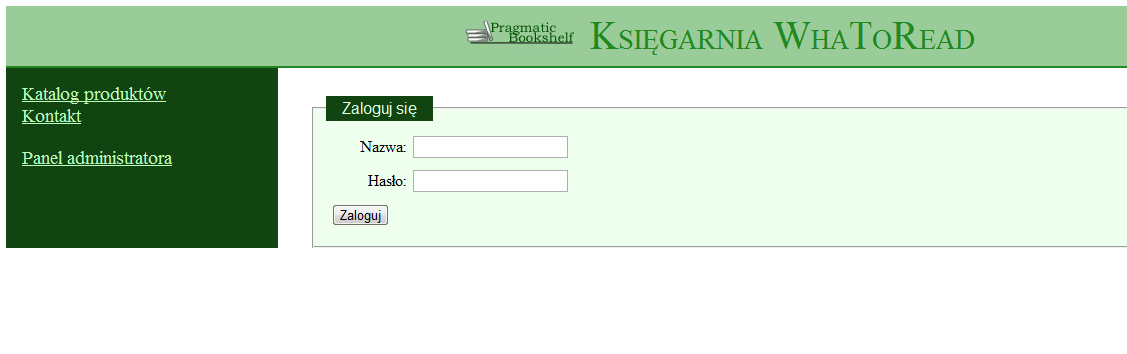
\includegraphics[width=\textwidth]{logowanie}
\caption{Logowanie}
\label{fig:logowanie}
\end{figure}

%\clearpage

%-------------------------

\section{Lista produktów}

\begin{figure}[!h]
\centering
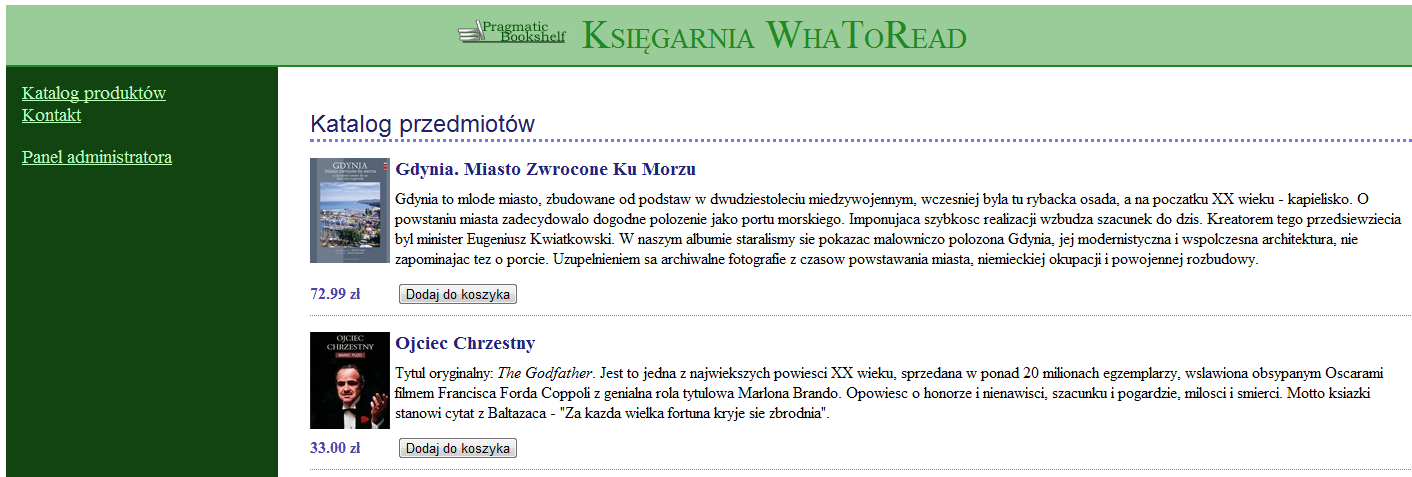
\includegraphics[width=\textwidth]{lista_produktow}
\caption{Lista produktów}
\label{fig:lista_produktow}
\end{figure}

\clearpage

%-------------------------

\section{Koszyk}

\begin{figure}[!h]
\centering
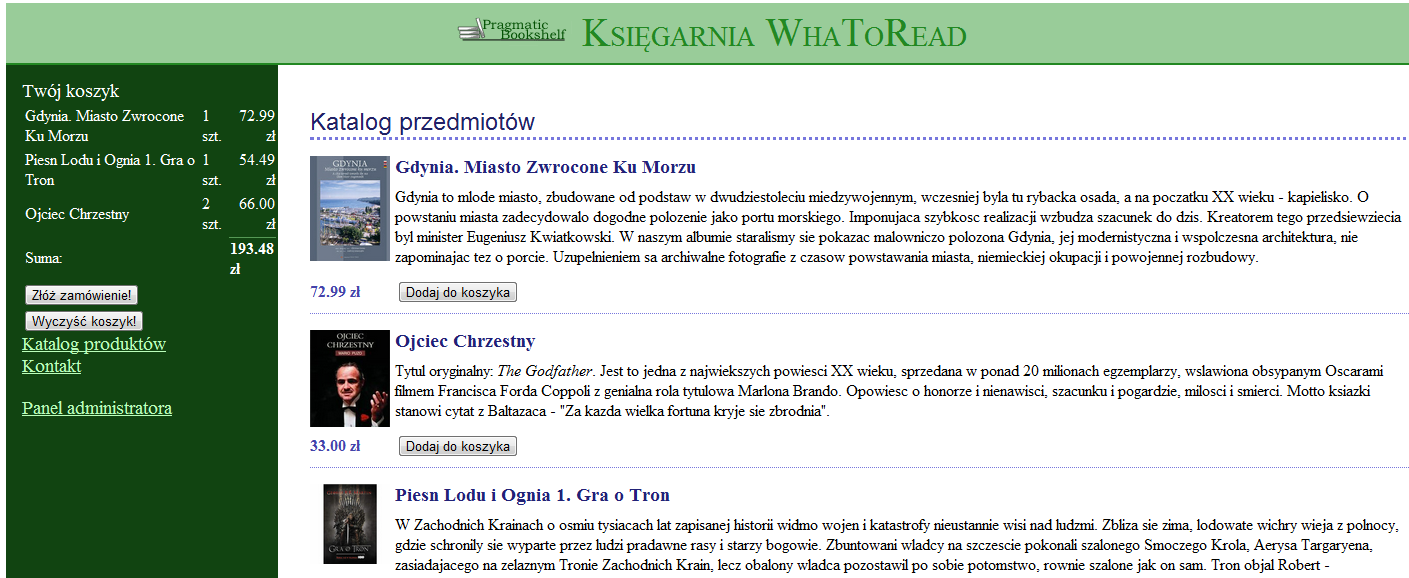
\includegraphics[width=\textwidth]{koszyk}
\caption{Koszyk}
\label{fig:koszyk}
\end{figure}

%-------------------------

\section{Zamówienie}

\begin{figure}[!h]
\centering
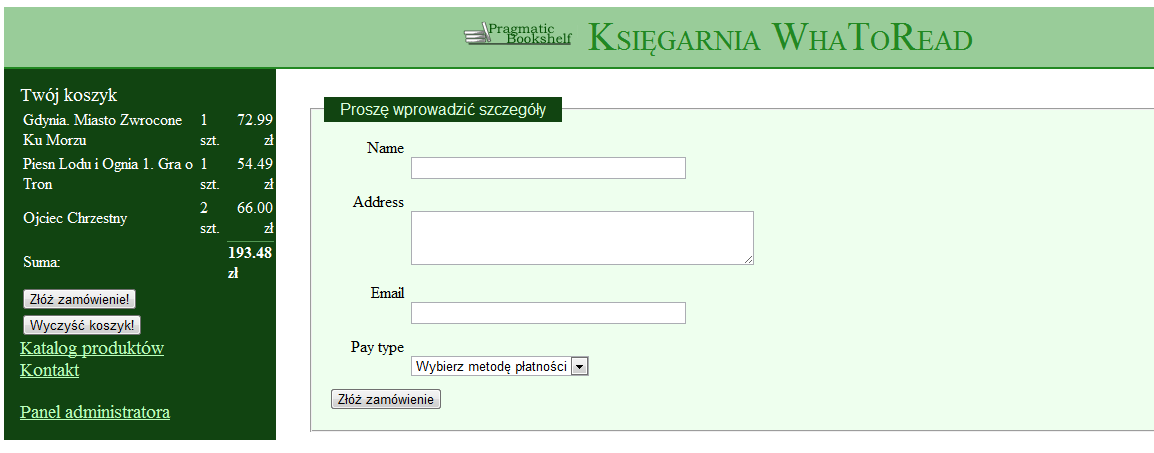
\includegraphics[width=\textwidth]{zamowienie_puste}
\caption{Zamówienie. Puste}
\label{fig:zamowienie_puste}
\end{figure}

\clearpage

%-------------------------

\begin{figure}[!h]
\centering
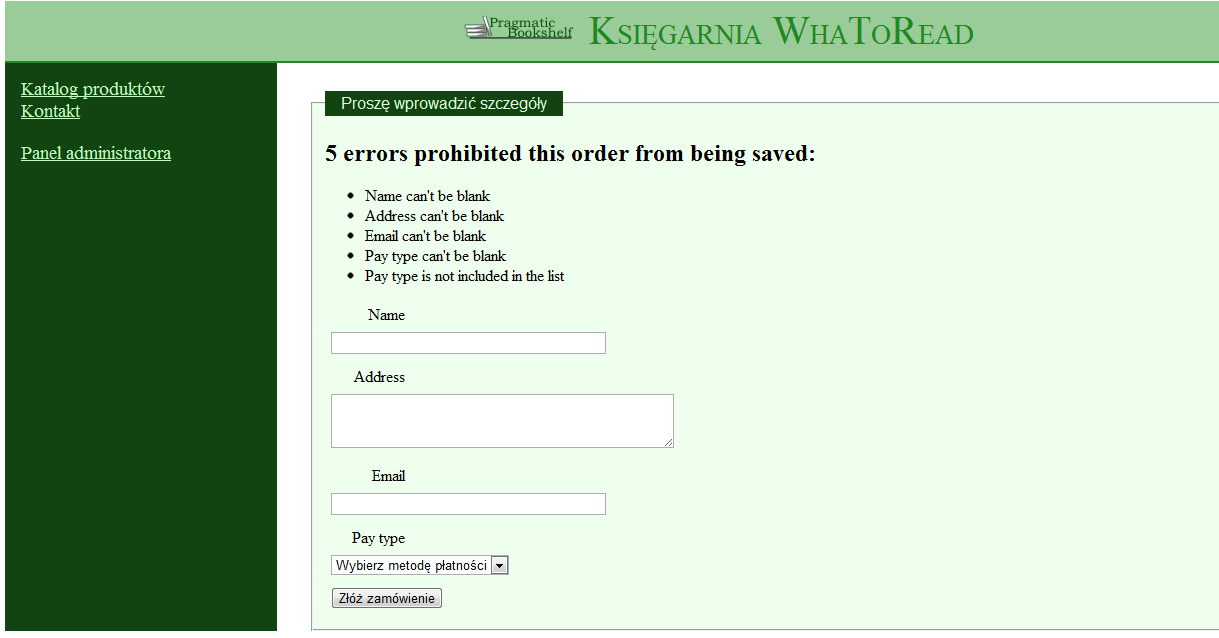
\includegraphics[width=\textwidth]{zamowienie_walidacja}
\caption{Zamówienie. Walidacja}
\label{fig:zamowienie_walidacja}
\end{figure}

%-------------------------

\begin{figure}[!h]
\centering
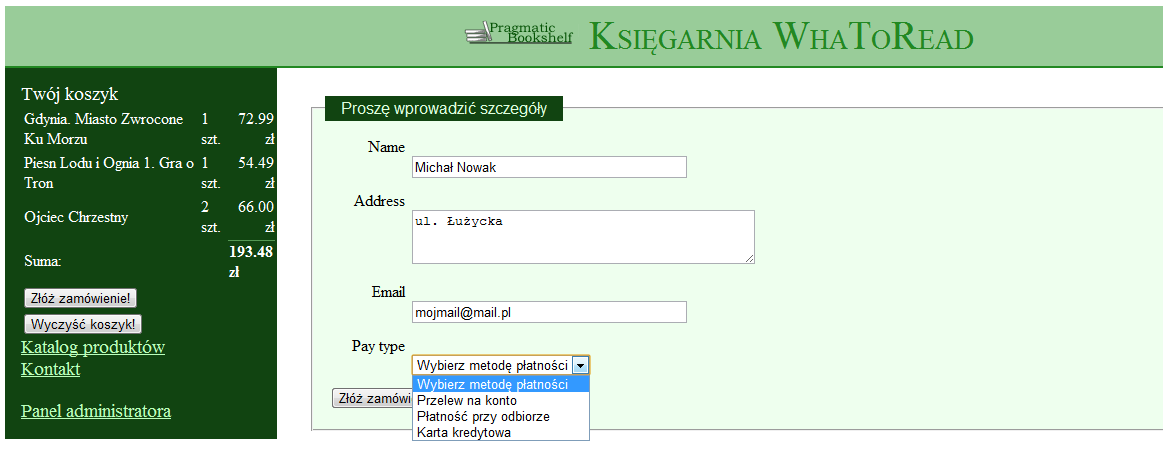
\includegraphics[width=\textwidth]{zamowienie_wypelnione}
\caption{Zamówienie. Wypełnione}
\label{fig:zamowienie_wypelnione}
\end{figure}

\clearpage

%-------------------------

\section{Administracja}

\begin{figure}[!h]
\centering
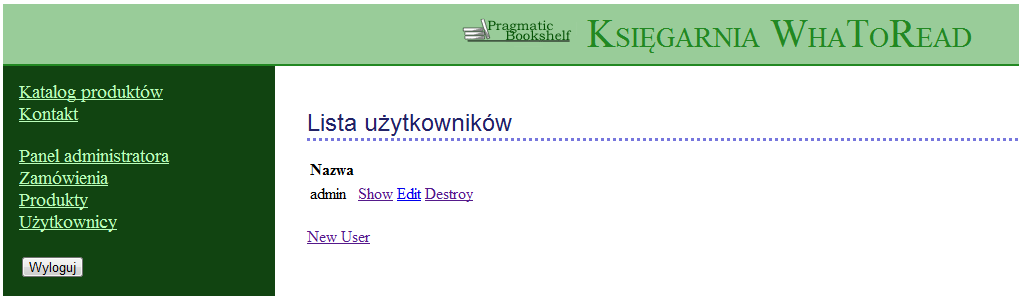
\includegraphics[width=\textwidth]{admin_uzytkownicy}
\caption{Administracja. Lista użytkowników}
\label{fig:admin_uzytkownicy}
\end{figure}

%-------------------------

\begin{figure}[!h]
\centering
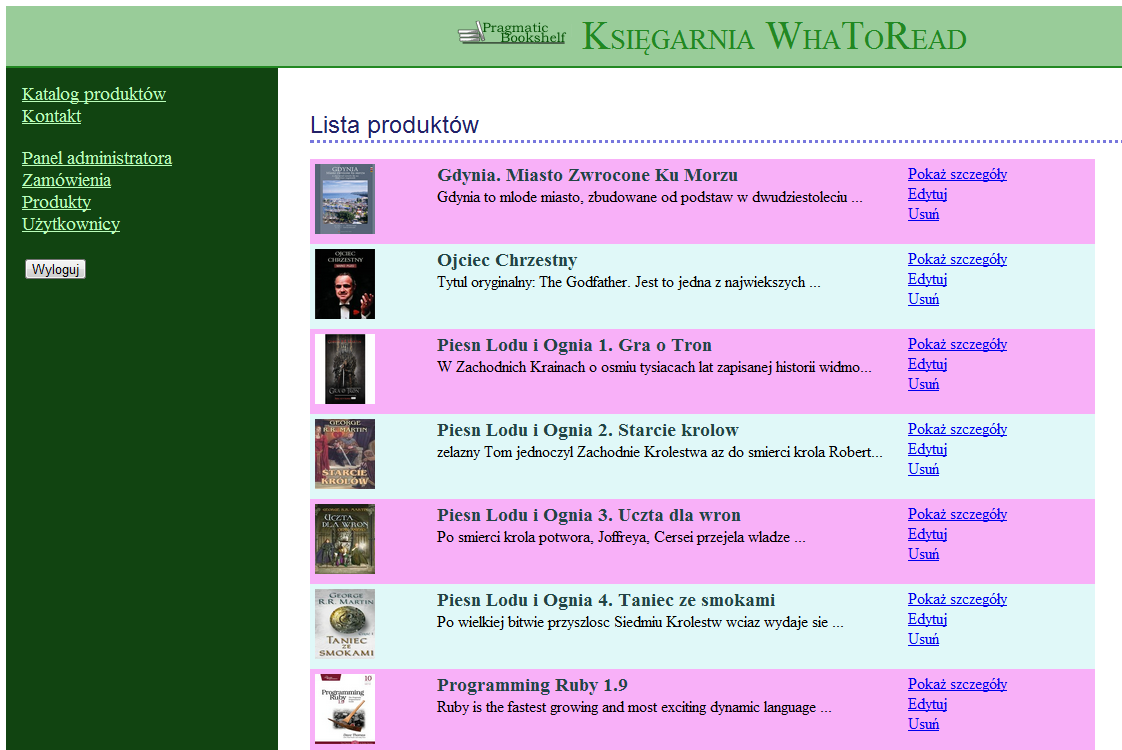
\includegraphics[width=\textwidth]{admin_produkty}
\caption{Administracja. Lista produktów}
\label{fig:admin_produkty}
\end{figure}

\clearpage

%-------------------------

\begin{figure}[!h]
\centering
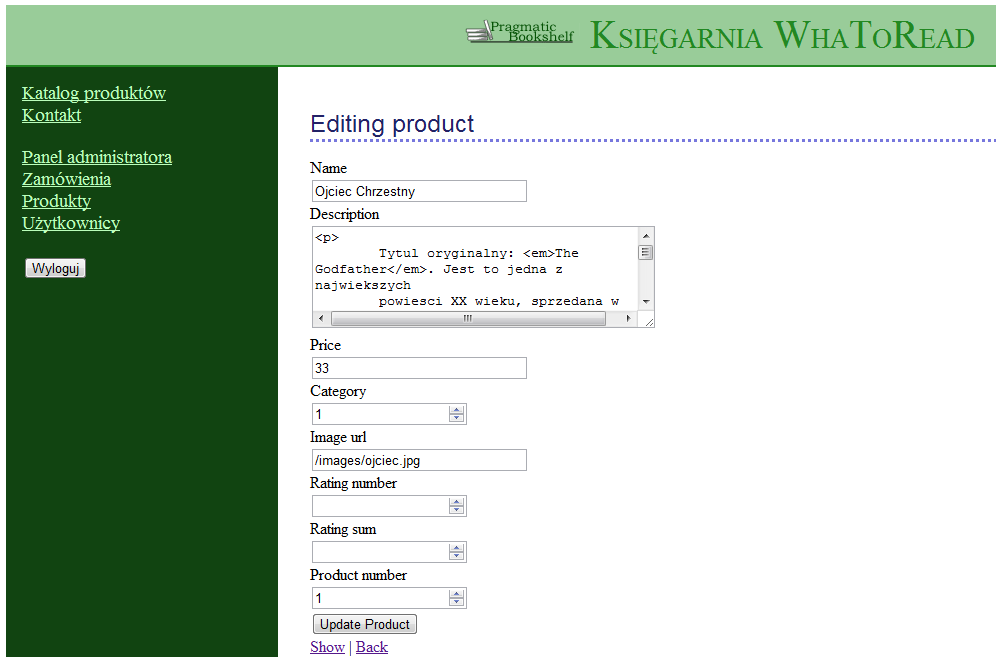
\includegraphics[width=\textwidth]{admin_edycja_produktu}
\caption{Administracja. Edycja produktu}
\label{fig:admin_edycja_produktu}
\end{figure}

%-------------------------

\begin{figure}[!h]
\centering
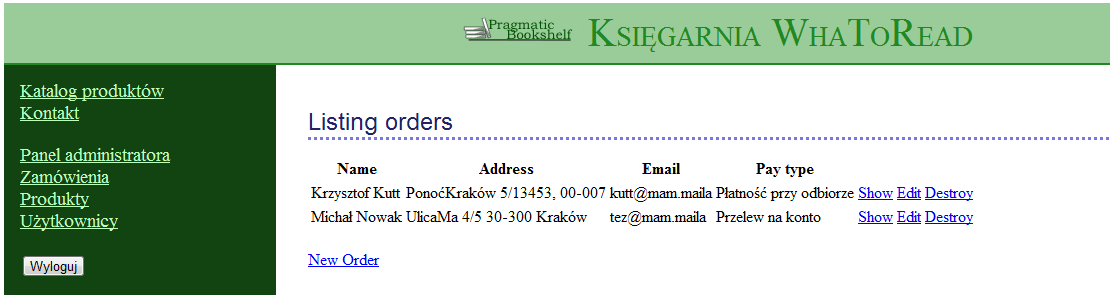
\includegraphics[width=\textwidth]{admin_zamowienia}
\caption{Administracja. Lista zamówień}
\label{fig:admin_zamowienia}
\end{figure}




\end{document}

